\documentclass[10pt,twocolumn]{article}

\usepackage[margin=0.72in]{geometry}
\usepackage{times}
\usepackage{microtype}
\usepackage{booktabs}
\usepackage{graphicx}
\usepackage{amsmath}
\usepackage{amssymb}
\usepackage{xcolor}
\usepackage{enumitem}
\usepackage{caption}
\usepackage{subcaption}
\usepackage[numbers,sort&compress]{natbib}
\usepackage[colorlinks=true,linkcolor=black,citecolor=blue!45!black,urlcolor=blue!45!black]{hyperref}

\definecolor{paperblue}{HTML}{1F4E79}
\definecolor{paperorange}{HTML}{C45A11}
\definecolor{papergray}{HTML}{4B5563}

\setlist[itemize]{leftmargin=*,topsep=2pt,itemsep=1pt}
\setlist[enumerate]{leftmargin=*,topsep=2pt,itemsep=1pt}
\captionsetup{font=small,labelfont=bf}

\newcommand{\method}{Chimera}
\newcommand{\artifacttps}{artifact tokens/s}
\newcommand{\modeltps}{model output tokens/s}

\title{\vspace{-0.35in}\bfseries Stop Generating the Code You Already Have:\\
\large Chimera Shared Edit Programs for Faster Long-Context Code Editing}

\author{
Ceyhun Derinbogaz
}

\date{May 28, 2026}

\begin{document}
\maketitle

\begin{abstract}
Modern LLM serving stacks are optimized around the decode loop: generate the
next token faster, schedule KV cache more efficiently, or speculate multiple
tokens ahead. For coding agents, this leaves a large systems opportunity
untouched. When the desired output is mostly a deterministic transformation of
context already available to the client, the model should not be asked to
regenerate the artifact token by token. We evaluate \method{} shared edit
programs, a compact validated representation for long-context code edits. On
50 deterministic LongCodeBench-derived 100K-context file-edit episodes using
Qwen/Qwen3.6-35B-A3B-FP8 served by vLLM 0.21.0 on a single H100, \method{}
achieves a \textbf{1.78$\times$ mean paired artifact-throughput speedup} over a
minimal unified-diff baseline under normal vLLM, with 95\% bootstrap CI
[1.56$\times$, 2.02$\times$]. Under vLLM Qwen MTP speculative decoding, the
same representation achieves \textbf{1.43$\times$} mean paired speedup over MTP
unified diff, with 95\% CI [1.26$\times$, 1.61$\times$]. All measured workloads
render successfully for all 50 examples. The result is deliberately narrow:
\method{} does not make the transformer emit raw tokens faster. It makes the
system produce the final edited artifact faster by emitting fewer redundant
tokens and rendering the rest deterministically.
\end{abstract}

\section{The Decode Tax Nobody Talks About}

LLM serving has become an arms race around the decode loop. vLLM introduced
PagedAttention for efficient serving memory management~\citep{kwon2023pagedattention}.
Speculative decoding~\citep{leviathan2023speculative} and multi-token
prediction~\citep{gloeckle2024mtp} attempt to accept several future tokens per
target-model step. These are real systems improvements.

But coding assistants often pay a tax before these optimizations matter: they
ask the model to repeat information that already exists in the client. A
file-edit assistant may receive a repository, identify a simple operation, and
then emit thousands of tokens of file content or patch scaffolding whose
semantics are mostly ``copy the existing text and add this small change.'' In
that regime, the right question is not only how fast the model decodes tokens.
It is why the model is decoding those tokens at all.

\method{} is a representation-level answer. The model emits a small validated
edit program. The client applies it. The artifact appears without forcing the
model to recite it.

\section{Method}

For copy-heavy code edits, the output artifact can be decomposed into large
substrings already present in context, small novel edits, and a deterministic
transformation that combines the two. Traditional full-file generation collapses
all three into raw text generation. Unified diff improves the situation by
emitting a patch. \method{} shared edit programs factor repeated operations
across files.

The operation evaluated here is intentionally simple:
\begin{verbatim}
{
  "operation": "prepend_many",
  "paths": ["file_a.py", "file_b.py",
            "file_c.py", "file_d.py"],
  "text": "# CHIMERA_EDIT_MARKER: ...\n"
}
\end{verbatim}

The client validates JSON parseability, operation type, exact path set, and
exact inserted text. It then renders the final edited files from source
artifacts already known to the harness. This is not a replacement for vLLM,
MTP, or KV-cache optimization. It is a layer above them: engine-level
acceleration asks the server to generate tokens faster; \method{} asks the
model to generate fewer tokens that better describe the operation.

\section{Experimental Setup}

\paragraph{Hardware and runtime.}
Experiments run on a Nebius \texttt{gpu-h100-sxm} VM with 1 NVIDIA H100 80GB
HBM3 GPU, driver 580.126.09, Qwen/Qwen3.6-35B-A3B-FP8~\citep{qwen36fp8}, and
vLLM 0.21.0~\citep{vllm}. The server uses max model length 131072, prefix
caching, chunked prefill, \texttt{MAX\_NUM\_SEQS=1}, and
\texttt{MAX\_NUM\_BATCHED\_TOKENS=8192}. Decoding uses temperature 0.0 and
top-$p$ 1.0.

\paragraph{Workload.}
We build 50 deterministic file-edit episodes from LongCodeBench LongCodeQA
\citep{longcodebench2025}. The first user turn contains approximately 96K Qwen
tokens of repository context. Each episode then asks the model to edit four
target files by prepending the same marker line. The source rows are
deterministically shuffled with seed 20260527. Every compared representation
uses the same record IDs and target files.

\paragraph{Compared systems.}
We compare normal vLLM and vLLM Qwen MTP with two output representations:
minimal unified diff and \method{} shared edit programs. We also include MTP
depth 6 because an earlier chat-style sweep favored it; in this edit workload,
depth 6 is slower than depth 2.

\paragraph{Metrics.}
\modeltps{} measures emitted model tokens per second. \artifacttps{} measures
validated final edited-file tokens per wall-clock second. \method{} is designed
to improve \artifacttps{}, not \modeltps{}.

\section{Results}

\begin{figure*}[t]
  \centering
  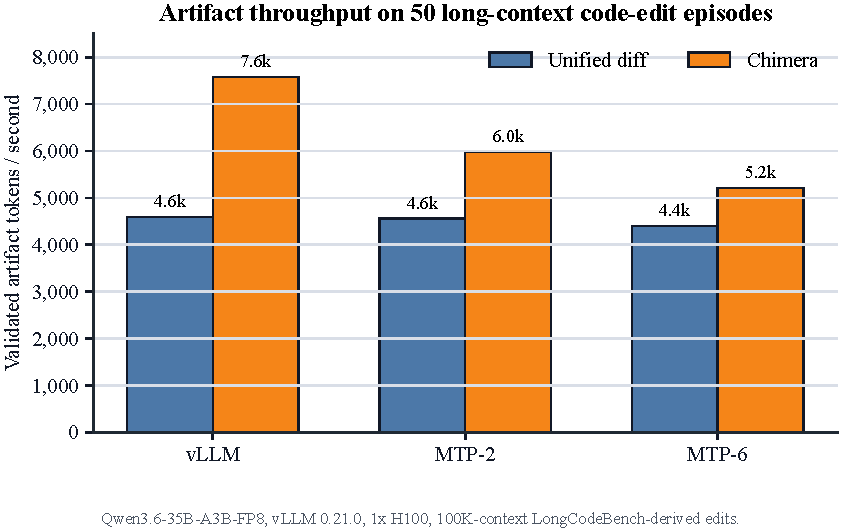
\includegraphics[width=0.94\textwidth]{figures/artifact_throughput.pdf}
  \caption{\textbf{Validated artifact throughput.} \method{} shared edit
  programs produce the same validated edited artifacts faster than minimal
  unified diff under both normal vLLM and MTP.}
  \label{fig:throughput}
\end{figure*}

\begin{table}[t]
\centering
\caption{Aggregate 50-example results. Every workload renders successfully for
all 50 examples.}
\label{tab:aggregate}
\resizebox{\columnwidth}{!}{%
\begin{tabular}{llrrrr}
\toprule
Profile & Workload & Render & Artifact tok/s & Output tok/s & Avg s\\
\midrule
vLLM & diff & 50/50 & 4586.19 & 65.47 & 2.62\\
vLLM & \method{} & 50/50 & 7576.24 & 41.87 & 1.59\\
MTP-2 & diff & 50/50 & 4555.04 & 65.03 & 2.64\\
MTP-2 & \method{} & 50/50 & 5982.65 & 33.06 & 2.01\\
MTP-6 & diff & 50/50 & 4393.81 & 62.73 & 2.74\\
MTP-6 & \method{} & 50/50 & 5208.69 & 28.79 & 2.31\\
\bottomrule
\end{tabular}}
\end{table}

\begin{figure}[t]
  \centering
  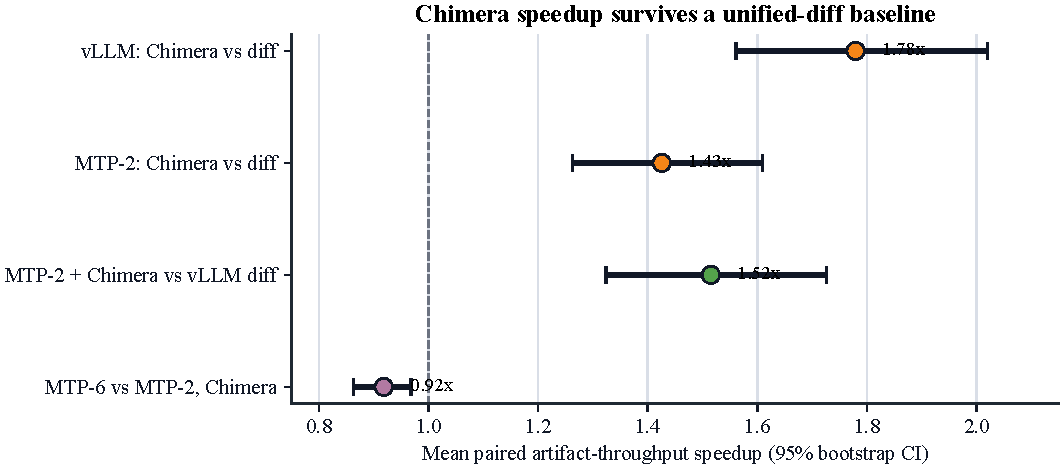
\includegraphics[width=\columnwidth]{figures/paired_speedups.pdf}
  \caption{\textbf{Paired per-example speedups.} Error bars show 95\%
  bootstrap confidence intervals over matching record IDs.}
  \label{fig:speedups}
\end{figure}

\begin{figure}[t]
  \centering
  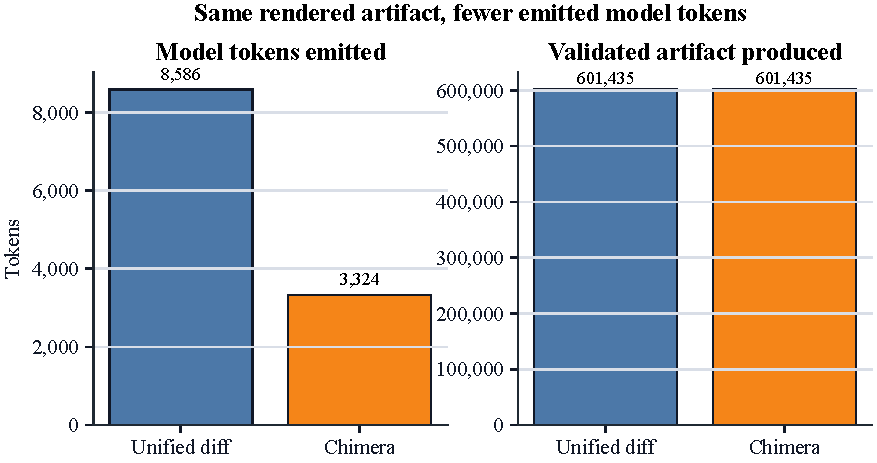
\includegraphics[width=\columnwidth]{figures/token_accounting.pdf}
  \caption{\textbf{Same artifact, fewer emitted tokens.} \method{} improves
  artifact throughput by reducing redundant output generation; it does not claim
  faster raw token emission.}
  \label{fig:tokens}
\end{figure}

The strongest result is not that \method{} beats a weak full-file baseline. It
beats a practical patch baseline. Against minimal unified diff, \method{}
improves effective artifact throughput by 1.78$\times$ on normal vLLM and by
1.43$\times$ when MTP is enabled. The speedup survives both a real patch-format
baseline and an engine-level speculative decoding control.

MTP is not a free win on this workload. Depth 2 slightly underperforms normal
vLLM in aggregate artifact throughput, and depth 6 is slower than depth 2. This
does not contradict earlier chat-trace measurements where MTP helped; it shows
that speculative settings do not automatically transfer to copy-heavy
edit-program workloads.

\section{Discussion}

\method{} wins here because the edit is shared across several files. Unified
diff is already compact, but it repeats file-level patch structure. \method{}
emits the operation once and points it at multiple paths. This distinction is
small in syntax and large in systems behavior.

This is not KV caching. KV caching avoids recomputing past context; it does not
stop the model from emitting redundant output tokens. This is not simply MTP
either. MTP tries to traverse the token sequence faster. \method{} shortens the
required sequence. The two ideas can be complementary, but this run shows they
are not guaranteed to compose positively without workload-specific tuning.

\begin{figure}[t]
  \centering
  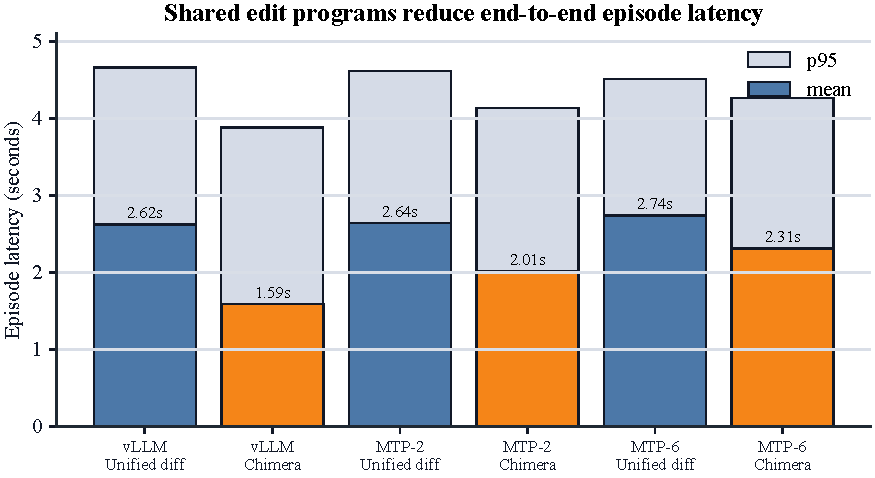
\includegraphics[width=\columnwidth]{figures/latency.pdf}
  \caption{\textbf{Episode latency.} Bars show mean latency; gray background
  bars show p95.}
  \label{fig:latency}
\end{figure}

\section{Limitations}

This is a systems result, not a universal model-quality result. It uses one
model, one engine, one GPU class, one concurrency setting, and one deterministic
edit family. The task intentionally isolates copy-render behavior; it does not
measure arbitrary reasoning-heavy software engineering. The correct claim is
that validated structured edit programs can improve artifact-level throughput
for copy-heavy code edits. The incorrect claim would be that the transformer
itself decodes raw tokens faster.

\section{Conclusion}

The usual inference story says faster LLM systems need faster kernels, better
KV-cache management, or speculative decoding. Those are real wins. This paper
shows another path: stop generating the artifact when a validated program can
render it.

On 50 LongCodeBench-derived 100K-context file-edit episodes, \method{} shared
edit programs deliver a 1.78$\times$ mean paired artifact-throughput speedup
over minimal unified diff on normal vLLM and a 1.43$\times$ speedup under MTP.
For coding agents, the next major speedup may not come from making models type
faster. It may come from teaching them when to stop typing.

\section*{Reproducibility}

The repository includes raw CSV summaries in \texttt{data/}, figure generation
in \texttt{scripts/make\_figures.py}, and a \texttt{Makefile}. The companion
experiment repository contains the raw per-request logs, generated traces, and
driver logs for the paper50 run.

\section*{AI Assistance Disclosure}

GPT-5.5 was used as an AI assistance tool during research planning, experiment
documentation, code and script drafting, figure preparation, and manuscript
editing. The named human author reviewed the experimental claims, source code,
figures, citations, and final manuscript, and remains responsible for the
content of this work.

\bibliographystyle{plainnat}
\bibliography{references}

\end{document}
